\documentclass[a4paper]{article}

\usepackage{tikz}
\usetikzlibrary{positioning}

\title{PaperTrader Protocol Specification}
\author{altffour}
\date{\today}

\begin{document}
\maketitle
\tableofcontents
\newpage

\section{Introduction}
This is the document for the specification of PaperTrader. PaperTrader is an
application for 'fake' trading assets, to practice investing. The document
contains explainations on how to implement the papertrader application. It 
should be noted that the document isn't `production-ready' until this sentence 
is removed. The document will go over the roles of the master server, and the
worker servers, how they interact with eachother and the communication protocol,
and finally, suggestions on server side implementations.

\section{Overview}
This section contains the required terminology and modelling of the PaperTrader
infrastructure.

\subsection{Terminology}

\subsubsection{Inner World}
This is Master server, and all worker servers. This should be kept under high
lockdown. Meaning, critical data should be kept secure.

\subsubsection{Outer World}
This is the frontend, including the desktop cleint, mobile client, or the
website client. The data here is controlled by the authorization of the account.

\subsubsection{Critical Data}
Cirtical Data are all data types that shouldn't be tampered with without
authorization. For example, accounts, personal information, messages, and in
this context user's portfolios.

\subsubsection{User/Client}
In this context it is the frontend, which is either the desktop client,
mobile client, or the website client.

\subsubsection{User/Client Data}
This is the data of the user. The meaning depends on the specific conext. It
could mean the personal information, credentials, etc. Most of the time it means
data that is attached to a data transfer to identify client (IP?).

\subsubsection{Master Server}
This is the main server that MUST be run when deploying the application.
Contains critical data, it would only interact to the outside world by the
worker servers.

\subsubsection{Worker Servers}
These are servers that contact the outer world. Worker Servers will
interact with the Master Server acting like a `cache' servers. Data should be 
routed through worker servers to the master server. The main job for worker 
server is to add timestamps onto commands sent from the user. The data sent to
the main server must contain the data of the client/user. There MUST be ATLEAST
one instance running to have a functional infrastructure.

\subsubsection{User Accounts}
This is the account that abstractly is a the data structure that contains
information about hte user and their account.

\subsection{Infrastructure Model}
A fully deployed infrastructure cotains \emph{ONE} master server, 
\emph{ATLEAST} one worker server, theoretically across the world to maintain 
speed and reliabilty. An overview diagram of the infrastructure: \newline

\begin{center}
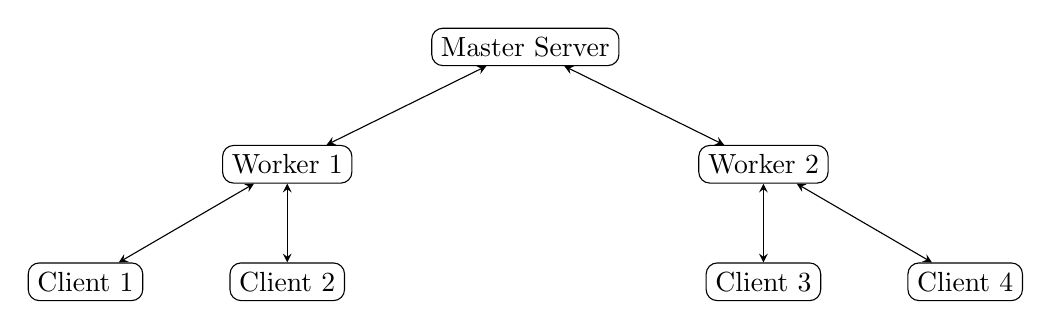
\begin{tikzpicture}[>=stealth,every node/.style={shape=rectangle,draw,rounded 
	corners}]
    % create the nodes
    \node (master) {Master Server};
    \node (worker1) [below left=of master]{Worker 1};
    \node (worker2) [below right=of master]{Worker 2};
	\node (client1) [below left=of worker1]{Client 1};
	\node (client12) [below =of worker1]{Client 2};
	\node (client2) [below =of worker2]{Client 3};
	\node (client22) [below right=of worker2]{Client 4};
    % connect the nodes
    \draw[<->] (master) -- (worker1);
    \draw[<->] (master) -- (worker2);
    \draw[<->] (worker1) -- (client1);
    \draw[<->] (worker2) -- (client2);
    \draw[<->] (worker1) -- (client12);
    \draw[<->] (worker2) -- (client22);
\end{tikzpicture} 
\end{center}

\newpage
\subsubsection{Master Server Infrastructure Model}
The master can be defined into modules as demonstrated in the following diagram:
\newline

\begin{center}
	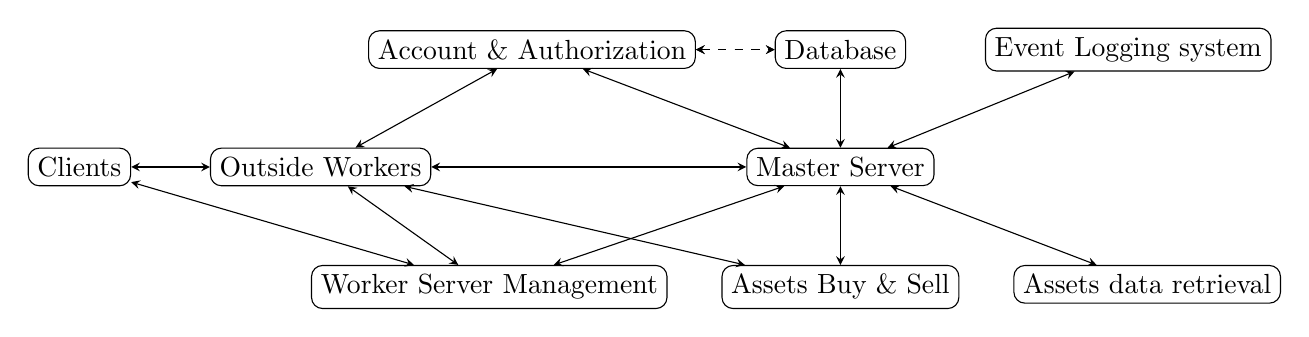
\begin{tikzpicture}[>=stealth,every node/.style={shape=rectangle,draw,rounded
		corners}]
		% create the nodes.
		\node (master) {Master Server};
		\node (db) [above=of master]{Database};
		\node (acc) [left=of db]{Account \& Authorization};
		\node (log) [right=of db]{Event Logging system};
		\node (worker) [below left=of master]{Worker Server Management};
		\node (asset) [below right=of master]{Assets data retrieval};
		\node (assettrans) [below=of master]{Assets Buy \& Sell};
		\node (outsideworkers) [left=4cm of master] {Outside Workers};
		\node (client) [left=of outsideworkers]{Clients};

		% connect the nodes
		\draw[<->] (outsideworkers) -- (master);
		\draw[<->] (master) -- (db);
		\draw[<->] (master) -- (acc);
		\draw[<->] (acc) -- (outsideworkers);
		\draw[<->, dashed] (acc) -- (db);
		\draw[<->] (master) -- (log);
		\draw[<->] (master) -- (worker);
		\draw[<->] (worker) -- (outsideworkers);
		\draw[<->, dashed] (acc) -- (db);
		\draw[<->] (master) -- (asset);
		\draw[<->] (master) -- (assettrans);
		\draw[<->] (assettrans) -- (outsideworkers);
		\draw[<->] (client) -- (worker);
		\draw[<->] (client) -- (outsideworkers);
	\end{tikzpicture}
\end{center}

\subsubsection{Worker Servers Infrastructure Model}
The worker servers can be defined into modules as demonstrated in the following
diagram:\newline

\begin{center}
	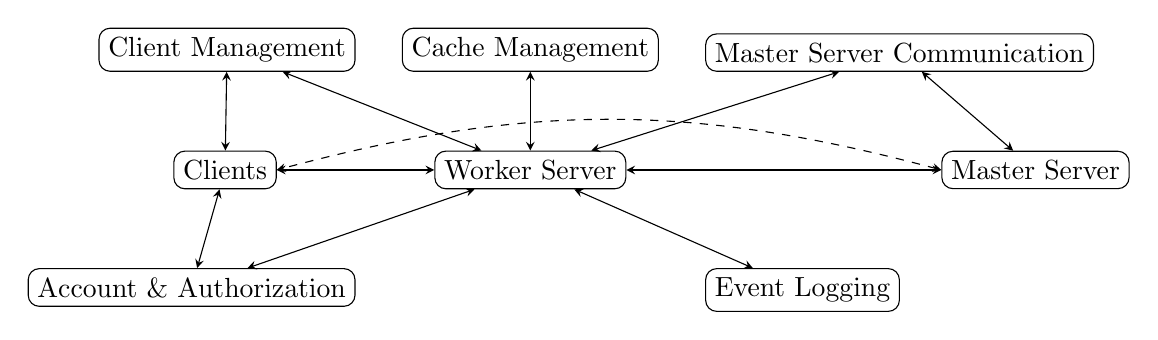
\begin{tikzpicture}[>=stealth,every node/.style={shape=rectangle,draw
		,rounded corners}]
		% create the nodes
		\node (workerserver) {Worker Server};
		\node (masterserver) [right=4cm of workerserver] {Master Server};
		\node (clients) [left=2cm of workerserver] {Clients};
		\node (mastercom) [above right=of workerserver] {Master Server 
			Communication};
		\node (cachemanage) [above=of workerserver] {Cache Management};
		\node (clientmanage) [above left=of workerserver] {Client Management};
		\node (accauth) [below left=of workerserver] {Account \& 
			Authorization};
		\node (event) [below right=of workerserver] {Event Logging};

		% connect the nodes
		\draw[<->] (masterserver) -- (workerserver);
		\draw[<->] (mastercom) -- (masterserver);
		\draw[<->] (workerserver) -- (clients);
		\draw[<->, dashed] (masterserver.west) to [bend right=15] 
		(clients.east);
		\draw[<->] (workerserver) -- (mastercom);
		\draw[<->] (workerserver) -- (cachemanage);
		\draw[<->] (workerserver) -- (clientmanage);
		\draw[<->] (clientmanage) -- (clients);
		\draw[<->] (workerserver) -- (accauth);
		\draw[<->] (accauth) -- (clients);
		\draw[<->] (workerserver) -- (event);

	\end{tikzpicture}
\end{center}

\subsection{Global Deployment Variables}
This section contains an overview of the global deployment variables.

\subsubsection{Number of Workers}
\label{var_num_worker}
This is the number of workers deployed with the master server. It must be 
atleast one. The worker server preferably should be deployed regionally.
\subsubsection{Memory Size of Log system}
\label{var_log_size}
This is a technical variable, this is the size of the log in memory before it 
being flushed to harddisk. Generally the smaller this is the more disk speed is
required. And the larger it is the more RAM the instance needs and the faster 
it is.
\subsubsection{Stock Data Update Interval}
\label{var_data_update_interval}
This is the interaval of the stock data retrieval. The more this is the faster
the transactions that can occur in a minute. This should be planned perfectly
so that it can maintain the userbase with the API calls.

\section{A more Technical Overview}
This is the section that describes the functioning parts of the project in
detail. We will start with modules, including master server modules, and worker
server modules.

\subsection{Master Server}
The master server has multiple modules:
\begin{itemize}
	\item Main Module, i.e the driver.
	\item Database Management.
	\item Account Management.
	\item Event Logging System.
	\item Worker Management.
	\item Assets Data Retrieval.
	\item Assets Transaction Management.
\end{itemize}

\subsubsection{Main Module}
\label{master_mods_main}
The main module should be able to do the following things:
\begin{itemize}
	\item Start the authorization thread.
	\item Start the Worker Management thread.
	\item Start the assets data retrieval thread.
	\item Start the assets transaction thread.
	\item Be able to parse commands from the worker threads.
	\item Be able to route the commands to the correct thread.
\end{itemize}

The main module's functionality in relation of the deployment and running stage
is as follows, The binary containing the master server is run -> initializes 
states required to operate the server -> start the threads -> start listening 
to workers -> parse it -> pass it to the appropriate thread. This is usually 
the set of functions that the main function would call. Putting the workings 
of the main module on a seperate is advised, since it gives the ability to
crash the server and dump the logs from the memory of the event log system.
Refer to \ref{var_log_size} for insight on why this is recommended.

\subsubsection{Database Management}
\label{master_mods_db}
The database management module sould be able to do the following things:
\begin{itemize}
	\item Be able to manipulate files (create, delete, write, read).
	\item Be able to convert data representations (structs) into SQL Databases.
\end{itemize}

The manipulations of files should be quite straightforward, a couple of
functions. The ability to access an SQL database is also necassery.

\subsubsection{Account Management \& Authorization}
\label{master_mods_acc}
The account management \& authorization module  should be able to do the 
following things:
\begin{itemize}
	\item Be able to register new users.
	\item Be able to login \emph{AND} authorize users.
	\item Be able to return a session token for the user.
	\item Be able to manage those session tokens.
\end{itemize}

The module should be able to take the set of information given and put them
into the database (using the database management \ref{master_mods_db}).
All passwords should be hashed and salted, this is up to the implementation on
the exact details. The accounts registered may contain third-party logins ex. 
Google Logins. In that case the account \emph{MUST} be recognized as an account
without a password, and the user should be asked to sign in with the 
third-party credentials. It should also be possible to add a password to the 
account marked to be 'logginable' with third-party logins, making it possible 
to login with the password and using third-party logins.

\subsubsection{Log System}
The log system should be able to do the following things:
\begin{itemize}
	\item To capture the date and time.
	\item To capture the caller's file, function, and line number.
	\item To capture a message and be able to format it.
	\item To be able to store it in a file.
\end{itemize}

One thing should be noted, the log system should not store in memory more 
entries than specified in the global variable: memory size of log system
(\ref{var_log_size}).

\end{document}
